\section{Maximum Mode Pins}
For using external coprocessors:
\begin{description}

    \item[$\overline{S2} , \overline{S1} and \overline{S0} $]
    \begin{itemize}
        \item Indicate the function of current bus-cycle
        \item Normally decoded by 8288 bus controllers
    \end{itemize}

    \item[$\overline{R1} / \overline{G1} and \overline{R0} / \overline{GT0} $]
    \begin{itemize}
        \item Request/grant pins
        \item Request Direct Memory Access
        \item Bi-Directional lines
        \item used to both request and grant a DMA operations
    \end{itemize}

    \item[$\overline{LOCK} $]
    \begin{itemize}
        \item Used to lock peripherals off the system
    \end{itemize}

    \item[$\overline{QS_1}  and \overline{QS0} $]
    \begin{itemize}
        \item Queue status bits
        \item Show status of the internal instructions queue
        \item Accessed by numeric coprocessor (8087)
    \end{itemize}

\end{description}

\begin{table}[h!]
\centering
\begin{tabular}{ |p{1cm}|p{1cm}|p{3cm}|  }
\hline
$ \overline{QS_1} $ & $ \overline{QS_0} $  & Function   \\
\hline
0 & 0 & Queue is idle \\
0 & 1 & First byte of opcode \\
1 & 0 & Queue is empty\\
1 & 1 & Subsequent byte of opcode \\
\hline
\end{tabular}

\caption{}
\label{table:4}
\end{table}

\section{Clock Generator (8284A)}
\begin{description}
  \item[Basic functions]
  \begin{itemize}
    \item Clock generation
    \item \textbf{RESET} synchronization
    \item READY synchronization
    \item TTL-level peripheral clock signal
  \end{itemize}
\end{description}
\newpage
\subsection{Pin diagram}
\begin{figure}[h!]
    \centering
    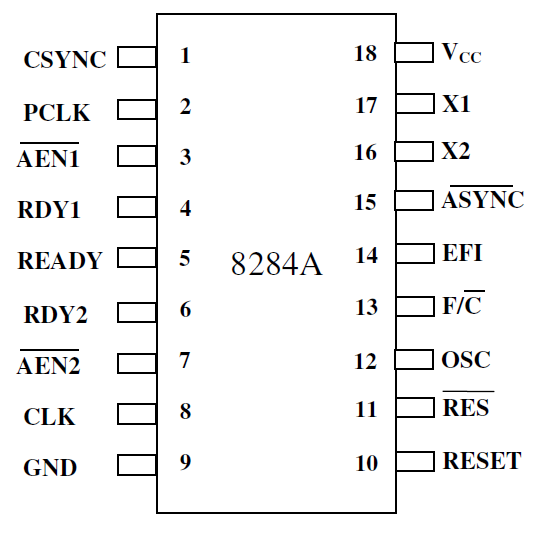
\includegraphics[width = 0.8\textwidth]{./figures/8284A.png}
    \caption{Pin Diagram for Intel 8284A}
    \label{fig:bl}
\end{figure}

\subsection{Pin Functions}
\begin{description}

  \item[AEN1 and AEN2]
  \begin{itemize}
    \item Qualify the bus ready signals, RDY1 and RDY2 respectively
    \item wait states are generated by the \textbf{READY} pin of $\mu P$, which is controlled
    by $\overline{AEN1}$ and $\overline{AEN2}$ pins
  \end{itemize}

  \item[RDY1 and RDY2]
  \begin{itemize}
    \item Bus ready inputs
    \item Cause wait states in conjunction with $\overline{AEN1}$ and $\overline{AEN2}$ pins
  \end{itemize}

  \item[$\overline{ASYNC}$]
  \begin{itemize}
    \item Ready synchronization
    \item Selects either one or two stages of synchronization for RDY1 and RDY2 inputs

  \end{itemize}

  \item[READY]
  \begin{itemize}
    \item An output pin that connects to the $\mu P's$ READY input
    \item Synchronized with RDY1 and RDY2 inputs
  \end{itemize}

\end{description}
